\documentclass[12pt]{article}

\usepackage[top=1in, bottom=1in, left=.75in, right=.75in]{geometry}
\usepackage{amsmath}
\usepackage{fancyhdr}
\usepackage{graphicx}
\usepackage{txfonts}
\usepackage{multicol,coordsys}
\usepackage[scaled=0.86]{helvet}
\renewcommand{\emph}[1]{\textsf{\textbf{#1}}}
\usepackage{anyfontsize}
\usepackage[shortlabels]{enumitem}
% \usepackage{times}
% \usepackage[lf]{MinionPro}
\usepackage{tikz,pgfplots,mathrsfs}
%\def\degC{{}^\circ{\rm C}}
\def\ra{\rightarrow}
\usetikzlibrary{calc, backgrounds}
\pgfplotsset{compat = newest}
\newcommand{\blank}[1]{\rule{#1}{0.75pt}}

\pgfplotsset{my style/.append style={axis x line=middle, axis y line=
middle, xlabel={$x$}, ylabel={$y$},axis equal}}

%yticklabels={,,} , xticklabels={,,}

% \setmainfont{Times}
% \def\sansfont{Lucida Grande Bold}
\parindent 0pt
\parskip 4pt
\pagestyle{fancy}
\fancyfoot[C]{\emph{\thepage}}
\fancyhead[L]{\ifnum \value{page} > 1\relax\emph{Math 252: Final Exam}\fi}
\fancyhead[R]{\ifnum \value{page} > 1\relax\emph{Spring 2024}\fi}
\headheight 15pt
\renewcommand{\headrulewidth}{0pt}
\renewcommand{\footrulewidth}{0pt}
\let\ds\displaystyle
\def\continued{{\emph {Continued....}}}
\def\continuing{{\emph {Problem \arabic{probcount} continued....}}\par\vskip 4pt}

\newcommand{\prob}[1]{\bigskip\noindent\textbf{#1.} }
\newcommand{\pts}[1]{{\small (\textsl{#1})}}

\newcommand{\probpts}[2]{\prob{#1} \pts{#2 pts} \quad}
\newcommand{\ppartpts}[2]{\textbf{(#1)} \pts{#2 pts} \quad}
\newcommand{\epartpts}[2]{\medskip\noindent \textbf{(#1)} \pts{#2 pts} \quad}


\begin{document}
{\emph{\fontsize{26}{28}\selectfont Math F252\hfill
{\fontsize{32}{36}\selectfont Final}
\hfill Spring 2024}}
\vskip 2cm
\strut\vtop{\halign{\emph#\hskip 0.5em\hfil&#\hbox to 4in{\hrulefill}\cr
\emph{\fontsize{18}{22}\selectfont Name:}&\cr
\noalign{\vskip 10pt}}}

\vspace{0.5in}
{\fontsize{18}{22}\selectfont\emph{Rules:}}

You have {2 hours} to complete this midterm.  

Partial credit will be awarded, but you must show your work.

Calculators and books are not allowed.  You may have 1/2 of a sheet of letter paper with notes.

Place a box around your \fbox{FINAL ANSWER} to each question.%, or use the box provided.

Turn off anything that might go beep during the exam.

Good luck!
\vfill
\def\emptybox{\hbox to 2em{\vrule height 16pt depth 8pt width 0pt\hfil}}
\def\tline{\noalign{\hrule}}
\centerline{\vbox{\offinterlineskip
{
\bf\sf\fontsize{18pt}{22pt}\selectfont
\hrule
\halign{
\vrule#&\strut\quad\hfil#\hfil\quad&\vrule#&\quad\hfil#\hfil\quad
&\vrule#&\quad\hfil#\hfil\quad&\vrule#\cr
height 3pt&\omit&&\omit&&\omit&\cr
&Problem&&Possible&&Score&\cr\tline
height 3pt&\omit&&\omit&&\omit&\cr
& 1&& 12&&\emptybox&\cr\tline
& 2&&  6&&\emptybox&\cr\tline
& 3&&  6&&\emptybox&\cr\tline
& 4&& 12&&\emptybox&\cr\tline
& 5&&  6&&\emptybox&\cr\tline
& 6&&  6&&\emptybox&\cr\tline
& 7&& 18&&\emptybox&\cr\tline
& 8&& 12&&\emptybox&\cr\tline
& 9&&  9&&\emptybox&\cr\tline
&10&& 15&&\emptybox&\cr\tline
&11&& 12&&\emptybox&\cr\tline
&12&& 11&&\emptybox&\cr\tline
&\textsl{Extra Credit}&& \textsl{3}&&\emptybox&\cr\tline
&Total&& 125&&\emptybox&\cr
}\hrule}}}

\newpage
\prob{1} On the axes below, sketch the region $R$ bounded by $y=2\sin(x)$ and $y=0$, between $x=0$ and $x=\pi.$ \\

\begin{tikzpicture}
\draw[ultra thick, ->] (-1,0) -- (5,0);
\draw[ultra thick, ->] (0,-1.5) -- (0,2.5);
\end{tikzpicture}

\epartpts{a}{6} Use an integral to find the volume  of the solid obtained by rotating $R$ about the $x$-axis.
\vfill

\epartpts{b}{6} Use an integral to find the volume  of the solid obtained by rotating $R$ about the $y$-axis.
\vfill

\newpage
\probpts{2}{6}  Find the area of the region $R$ in the plane bounded by $f(x)=\arctan(x)$, $y=0$ and $x=1.$ The graph of arctangent is provided below.  (\textsl{Hint. You will need to use a technique of integration.}) \\

\includegraphics[scale=.2]{arctan.png}
\vspace{2.0in}

\probpts{3}{6} Evaluate the sum $\displaystyle \sum_{n=0}^\infty \frac{3^{n+2}}{4^{n}}$.
\vfill


\newpage
\prob{4}  Evaluate the indefinite integrals below.

\epartpts{a}{6} $\displaystyle{\int \frac{\sqrt{x^2-4}}{x} \, dx}$ \hfill (\textsl{Hint. Substitute $x=2 \sec(\theta).$})
\vfill

\epartpts{b}{6} $\displaystyle{\int \sin^3(2\theta)\cos^4(2\theta) \, d\theta}$
\vfill

\newpage
\probpts{5}{6}  %A 2-meter spring requires 3 J to stretch the spring to a length of 2.1 meters. How much work would it take to stretch the spring from 2 meters to 2.3 meters?
A spring with a relaxed length of 2 meters requires 3 Newtons force to stretch to a length of 2.1 meters.  How much work would it take to stretch the spring from 2 meters to 2.3 meters?
\vfill

\probpts{6}{6}  Use the  Integral Test to determine if the series $\displaystyle \sum_{n=0}^\infty \frac{2n+e^n}{(n^2+e^n)^2}$ converges. Use correct limit notation.
\vfill

\newpage
\prob{7} \pts{6 pts each} \quad Do the following series converge or diverge? Show your work including \textbf{naming} any test you use.

\renewcommand{\labelenumi}{\textbf{(\alph{enumi})}}
	\begin{enumerate}[leftmargin=7mm]
	\item \, $\displaystyle{\sum_{n=1}^\infty \frac{n^{3/2}}{100n^2+20n}}$
	\vfill
	\item \, $\displaystyle{\sum_{n=2}^\infty \left(\frac{6n+5}{5n+10}\right)^n}$
	\vfill
	\item \, $\displaystyle{\sum_{n=0}^\infty \frac{(-1)^n}{\sqrt{2n+1}}}$
	\vfill
	\end{enumerate}

\newpage
\prob{8} \pts{6 pts each} \quad For each power series below determine the \emph{interval} of convergence.
	\begin{enumerate}[leftmargin=7mm]
	\item \,$\displaystyle \sum_{n=1}^\infty \frac{(3x)^n}{n^2}$
	\vfill
	\item \,$\displaystyle \sum_{n=1}^\infty \frac{(n-1)!(x-5)^n}{2n}$
	\vfill
	\end{enumerate}

\newpage
\prob{9} Let \,{\large $f(x)=\ln(x)$}. 
	\begin{enumerate}[leftmargin=7mm]
	\item \pts{3 pts} \, Find a formula for $f^{(n)}(x),$ the $n$th derivative of $f(x).$
	\vspace{3.0in}
	\item \pts{6 pts} \, Find the Taylor series for $f(x)$ centered at $a=1.$ Your answer should be reasonably simplified.
	\vfill
	\end{enumerate}

\newpage
\prob{10} Consider the curve defined by the parametric equations \hspace{.2in} {\large $x=e^t$, \hspace{.1in} $y=(t-1)^2$}.
	\begin{enumerate}[leftmargin=7mm]
	\item \pts{5 pts} \,  Determine the slope of the curve at the point $(1,1).$
	\vfill
	\item \pts{5 pts} \,  Determine the points on the curve at which the tangent line is horizontal or vertical, or state that none exist.
	\vfill
	\item \pts{5 pts} \,  Set up but do not evaluate an integral for the length of the curve from $t=1$ to $t=2.$
	\vfill
	\end{enumerate}  

\newpage
\prob{11} Recall the Maclaurin series $\displaystyle e^x = \sum_{n=0}^\infty \frac{x^n}{n!}.$
	\begin{enumerate}[leftmargin=7mm]
	\item \pts{3 pts} \,  Find the Maclaurin series for $\ds h(x)=xe^{-2x}.$  Your answer should be simplified.\\
	\vspace{1in}
	\item \pts{3 pts} \,  Determine the value of the convergent series \,$\ds \sum_{n=0}^\infty \frac{3^{2n}}{n!}$
	\vspace{1in}
	\item \pts{6 pts} \,  Find the Maclaurin series for \,$\ds F(x)=\int_0^x e^{-t^2} dt$
	\vfill
	\end{enumerate}

\newpage
\prob{12}  \ppartpts{a}{3} Convert the rectangular equation $y^2=5x$ to polar form.
\vspace{1.5in}

\epartpts{b}{3} Convert the polar equation $r=\sin \theta$ to rectangular form.
\vspace{1.5in}

\epartpts{c}{5} Sketch the polar curve $r=2+2\cos\theta.$\\

%%%%POLAR GRAPH	
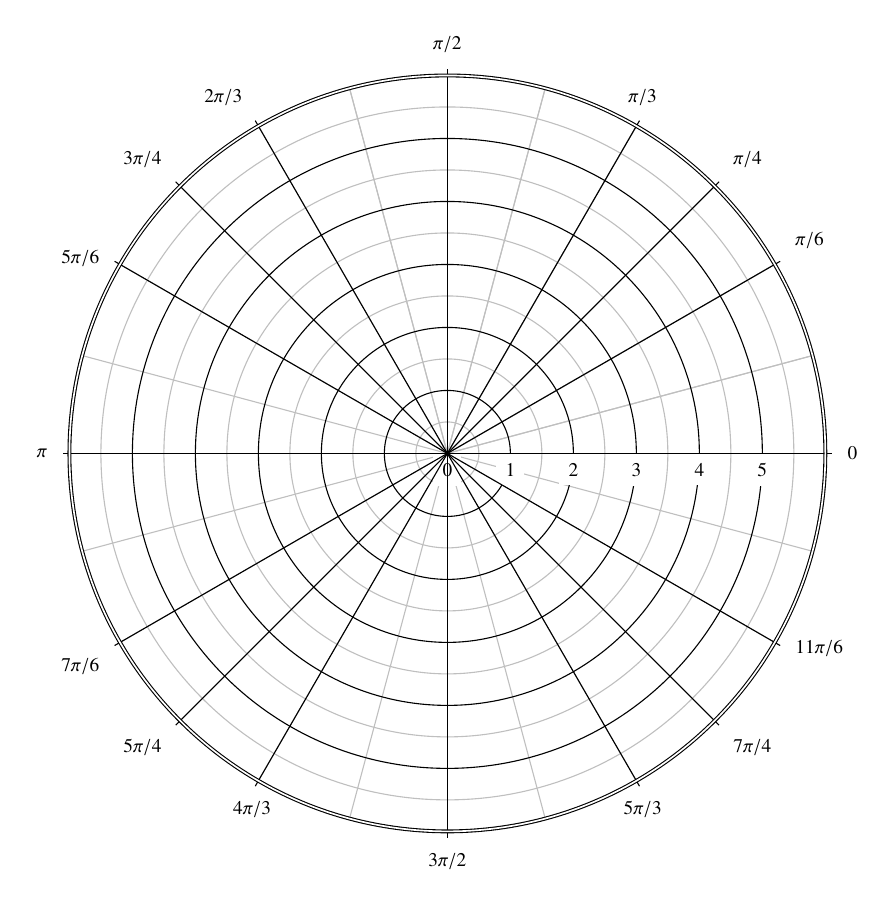
\begin{tikzpicture}[>=latex, scale=0.8]
% Draw the lines at multiples of pi/12
\foreach \ang in {0,...,31} {
  \draw [lightgray] (0,0) -- (\ang * 180 / 12:6);
}
% Concentric circles and radius labels
\foreach \s in {0, 1, 2, 3,4,5} {
  \draw [lightgray] (0,0) circle (\s + 0.5);
  \draw (0,0) circle (\s);
  \node [fill=white] at (\s, 0) [below] {\scriptsize $\s$};
}
% Add the labels at multiples of pi/4
\foreach \ang/\lab/\dir in {
  0/0/right,
  1/{\pi/4}/{above right},
  2/{\pi/2}/above,
  3/{3\pi/4}/{above left},
  4/{\pi}/left,
  5/{5\pi/4}/{below left},
  7/{7\pi/4}/{below right},
  6/{3\pi/2}/below} {
  \draw (0,0) -- (\ang * 180 / 4:6.1);
  \node [fill=white] at (\ang * 180 / 4:6.2) [\dir] {\scriptsize $\lab$};
}
% Add the labels at multiples of pi/6
\foreach \ang/\lab/\dir in {
  1/{\pi/6}/{above right},
  2/{\pi/3}/above,
  4/{2\pi/3}/{above left},
  5/{5\pi/6}/{left},
  7/{7\pi/6}/{below left},
  8/{4\pi/3}/below,
  10/{5\pi/3}/below,
  11/{11\pi/6}/right} {
  \draw (0,0) -- (\ang * 180 / 6:6.1);
  \node [fill=white] at (\ang * 180 / 6:6.2) [\dir] {\scriptsize $\lab$};
}
% The double-lined circle around the whole diagram
\draw [style=double] (0,0) circle (6);
\end{tikzpicture}

\clearpage\newpage
\probpts{Extra Credit}{3}  Determine the values of $p$ for which the series $\ds \sum_{n=2}^\infty \frac{1}{n (\ln n)^p}$ converges, and justify your answer.  Assume $p\ge 0$.
\vfill

\noindent\hrulefill

You may find the following \textbf{trigonometric formulas} useful.  Other formulas, not listed here, should be in your memory, or you can derive them from the ones here.
\begin{align*}
\sin(\alpha \pm \beta) &= \sin \alpha \cos \beta \pm \cos \alpha \sin \beta \qquad &
    \sin(ax) \sin(bx) &= \frac{1}{2} \cos((a-b)x) - \frac{1}{2} \cos((a+b)x) \\
\cos(\alpha \pm \beta) &= \cos \alpha \cos \beta \mp \sin \alpha \sin \beta \qquad &
    \sin(ax) \cos(bx) &= \frac{1}{2} \sin((a-b)x) + \frac{1}{2} \sin((a+b)x) \\
 && \cos(ax) \cos(bx) &= \frac{1}{2} \cos((a-b)x) + \frac{1}{2} \cos((a+b)x)
\end{align*}

\clearpage\newpage
\large\centerline{\textbf{Summary of Convergence Tests}}
\normalsize

\vspace{-2mm}
\begin{center}
\includegraphics[width=0.89\textwidth]{serieshandoutA.png}
\end{center}
\vfill


\clearpage\newpage
\begin{center}
\includegraphics[width=0.9\textwidth]{serieshandoutB.png}

\vspace{-2mm}
\includegraphics[width=0.9\textwidth]{serieshandoutC.png}
\end{center}
\vfill

\end{document}